\section{项目简介}

本章从项目提出背景与建设意义出发，概述系统的业务内容与功能边界，对国内外同类方案进行对比分析，并按用户角色梳理核心需求，为后续章节的建模与设计提供上下文依据。

\subsection{项目提出与意义}

\subsubsection{当前痛点}

当前，脑电图（EEG）数据在教学与基础科研场景中的管理现状不容乐观。一方面，大量实验室仍采用``文件夹 + 手工台账''的方式管理数据，实验记录、被试者信息与采集参数分散于不同媒介，缺乏统一的元数据标准和结构化的关联机制。另一方面，数据质量的把控高度依赖研究者的个人经验，从原始信号的格式校验、通道完整性检查到伪迹识别，缺少系统化的自动质控工具，导致下游分析结果的可靠性难以保证。

更为紧迫的是科研伦理审查的规范化缺失。涉及人类被试者的 EEG 实验本应遵循知情同意、数据最小化使用和隐私保护等基本原则，但在实际操作中，知情同意书多以纸质签署、扫描存档的方式管理，数据使用授权缺乏电子化审批流程，操作过程缺少不可篡改的日志记录。一旦面临科研诚信审查或合规检查，现有的管理方式难以提供完整、可追溯的证据链。

\subsubsection{需求现状}

上述困境并非孤立存在，而是多重因素叠加的结果。从政策层面看，《中华人民共和国数据安全法》（2021）和《中华人民共和国个人信息保护法》（2021）的相继实施，对涉及个人生物特征数据的采集、存储和使用提出了明确的合规要求。从学术规范层面看，越来越多的期刊和资助机构要求研究者遵循 FAIR 原则（Findable, Accessible, Interoperable, Reusable），对数据的可发现性、可访问性、互操作性和可复用性提出了系统性的要求。从教学层面看，高校神经科学和认知科学相关课程亟需一个贴近真实科研场景的教学平台，使学生在掌握 EEG 数据采集技术的同时，建立起规范的数据管理和伦理合规意识。

在此背景下，建设一套面向教学与基础科研场景的轻量级 EEG 数据管理与科研伦理审核系统，已成为支撑脑科学人才培养和科研基础设施建设的现实需求。

\subsubsection{建设意义}

本系统的建设具有以下三重意义：

\begin{enumerate}
  \item \textbf{提升科研数据管理水平}——通过统一的数据组织规范、自动化的解析质控流程和完整的生命周期管理机制，从根本上解决 EEG 数据``找不到、管不住、用不好''的难题，为科研数据的可复现性提供技术保障。
  \item \textbf{支撑科研伦理合规建设}——通过知情同意书的电子化管理、数据使用授权的线上审批、操作日志的全程留痕和数据脱敏机制，构建可审计、可追溯的伦理合规闭环，帮助科研团队建立符合法规要求的伦理审查实践。
  \item \textbf{赋能教学与人才培养}——以轻量化、低门槛的系统形态，为高校神经科学和软件工程课程提供兼具学科深度和工程实践价值的教学平台，让学生在真实的系统交互中理解数据治理与伦理审查的核心理念。
\end{enumerate}

\subsection{项目具体内容介绍}

\subsubsection{业务全景}

本系统围绕 EEG 数据的完整生命周期，覆盖从实验创建、数据采集入库、自动解析质控，到伦理审核授权、智能分析利用和数据归档的全链路业务。系统处理的核心对象包括：用户账号与角色信息、实验项目与元数据、EEG 原始数据文件与派生数据、知情同意模板与签署记录、数据使用申请与授权凭证、异步处理任务与分析结果，以及操作日志与系统配置。

核心业务流程可概括为以下主线：

\begin{enumerate}
  \item \textbf{实验归集}——实验员创建实验项目，录入实验元数据，上传 EEG 原始数据文件。
  \item \textbf{自动质控}——系统对上传的 EEG 文件自动执行格式解析、采样率校验、通道完整性检查、缺失值与异常值检测，生成质控报告。
  \item \textbf{伦理审核}——被试者完成知情同意书的电子化签署；实验员提交数据使用申请；管理员对数据合规性和使用授权进行审批。
  \item \textbf{分析利用}——经授权的实验员可对审核通过的数据执行时域波形分析、频域特征提取和 AI 状态识别等分析任务。
  \item \textbf{生命周期管理}——数据在``已上传 $\to$ 处理中 $\to$ 待审核 $\to$ 已通过 / 已拒绝 $\to$ 已冻结 $\to$ 已归档''的状态流转中完成全生命周期管理，每一步均留有操作日志。
\end{enumerate}

\subsubsection{系统定位与功能边界}

本系统定位于``轻量级''和``科研''两个核心属性，在功能设计上做出如下界定：

\textbf{包含范围}：用户注册与角色管理、实验与 EEG 数据的上传存储、自动解析与质控报告生成、知情同意模板管理与电子化签署、数据使用申请与授权审批流程、基本的 EEG 信号分析（时域波形、频谱分析、频段能量、AI 状态识别）、操作审计日志、系统运行参数配置、站内通知与消息推送。

\textbf{排除范围}：本系统不涉及 EEG 信号的高级源定位分析（如 LORETA、Beamformer）、不提供临床级别的诊断辅助功能、不承担真实伦理委员会（IRB）的法律审查职能、不支持大规模分布式数据集的联邦计算、不提供 EEG 硬件设备的驱动与实时采集控制。

在技术形态上，本系统采用 B/S（Browser/Server）架构，前端基于现代 Web 框架构建响应式用户界面，后端提供 RESTful API 接口，数据持久化层采用关系数据库，文件存储采用对象存储服务。系统整体追求轻量化部署——单服务器即可运行，无需依赖复杂的大数据基础设施或 GPU 集群，以降低基础科研的使用门槛。

\subsection{产品市场分析}

本节对国内外 EEG 数据管理与分析领域的代表性工具进行调研和对比，分析其优缺点及对本系统设计的借鉴意义。

\subsubsection{国外分析}

EEGLAB 是由加州大学圣迭戈分校开发的开源 MATLAB 工具箱，是目前 EEG 领域使用最广泛的数据分析平台之一。EEGLAB 提供了丰富的信号处理功能，包括独立成分分析（ICA）、事件相关电位（ERP）分析和时频分析等，拥有活跃的插件生态。然而，EEGLAB 以 MATLAB 为运行环境，授权成本高昂，对非计算机背景的初学者学习曲线陡峭；且其设计定位于单用户桌面分析，缺乏多用户协作、数据权限管理和伦理审核流程等面向团队科研管理的功能。

\begin{figure}[H]
  \centering
  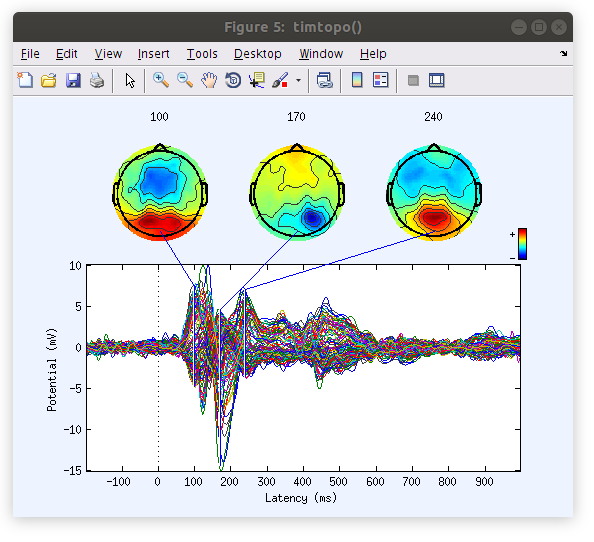
\includegraphics[width=0.65\textwidth]{figures/02_eeglab_example.png}
  \caption{EEGLAB 图形用户界面示例}
  \label{fig:eeglab-gui}
\end{figure}

MNE-Python 是基于 Python 的开源 EEG/MEG 分析框架，由哈佛医学院和法国国家健康与医学研究院（INSERM）共同维护。MNE-Python 在信号处理算法的丰富性和代码质量方面处于领先地位，支持 BIDS 数据标准的读写，具备良好的可编程性和可复现性。但其定位同样是专业级分析工具，以命令行和脚本交互为主，主要是以纯代码形式的开发套件，缺少面向教学场景的图形化操作界面，且同样不具备数据伦理审核和多用户权限管理能力。

OpenNeuro 是一个面向神经影像数据共享的开放平台，严格遵循 BIDS 标准，支持数据集的公开发布与复用。OpenNeuro 在数据标准化和开放共享方面提供了先进的实践范式，但其定位是数据存档与共享仓库，不提供数据分析、质控报告生成或伦理审核流程管理等功能。

\begin{figure}[H]
  \centering
  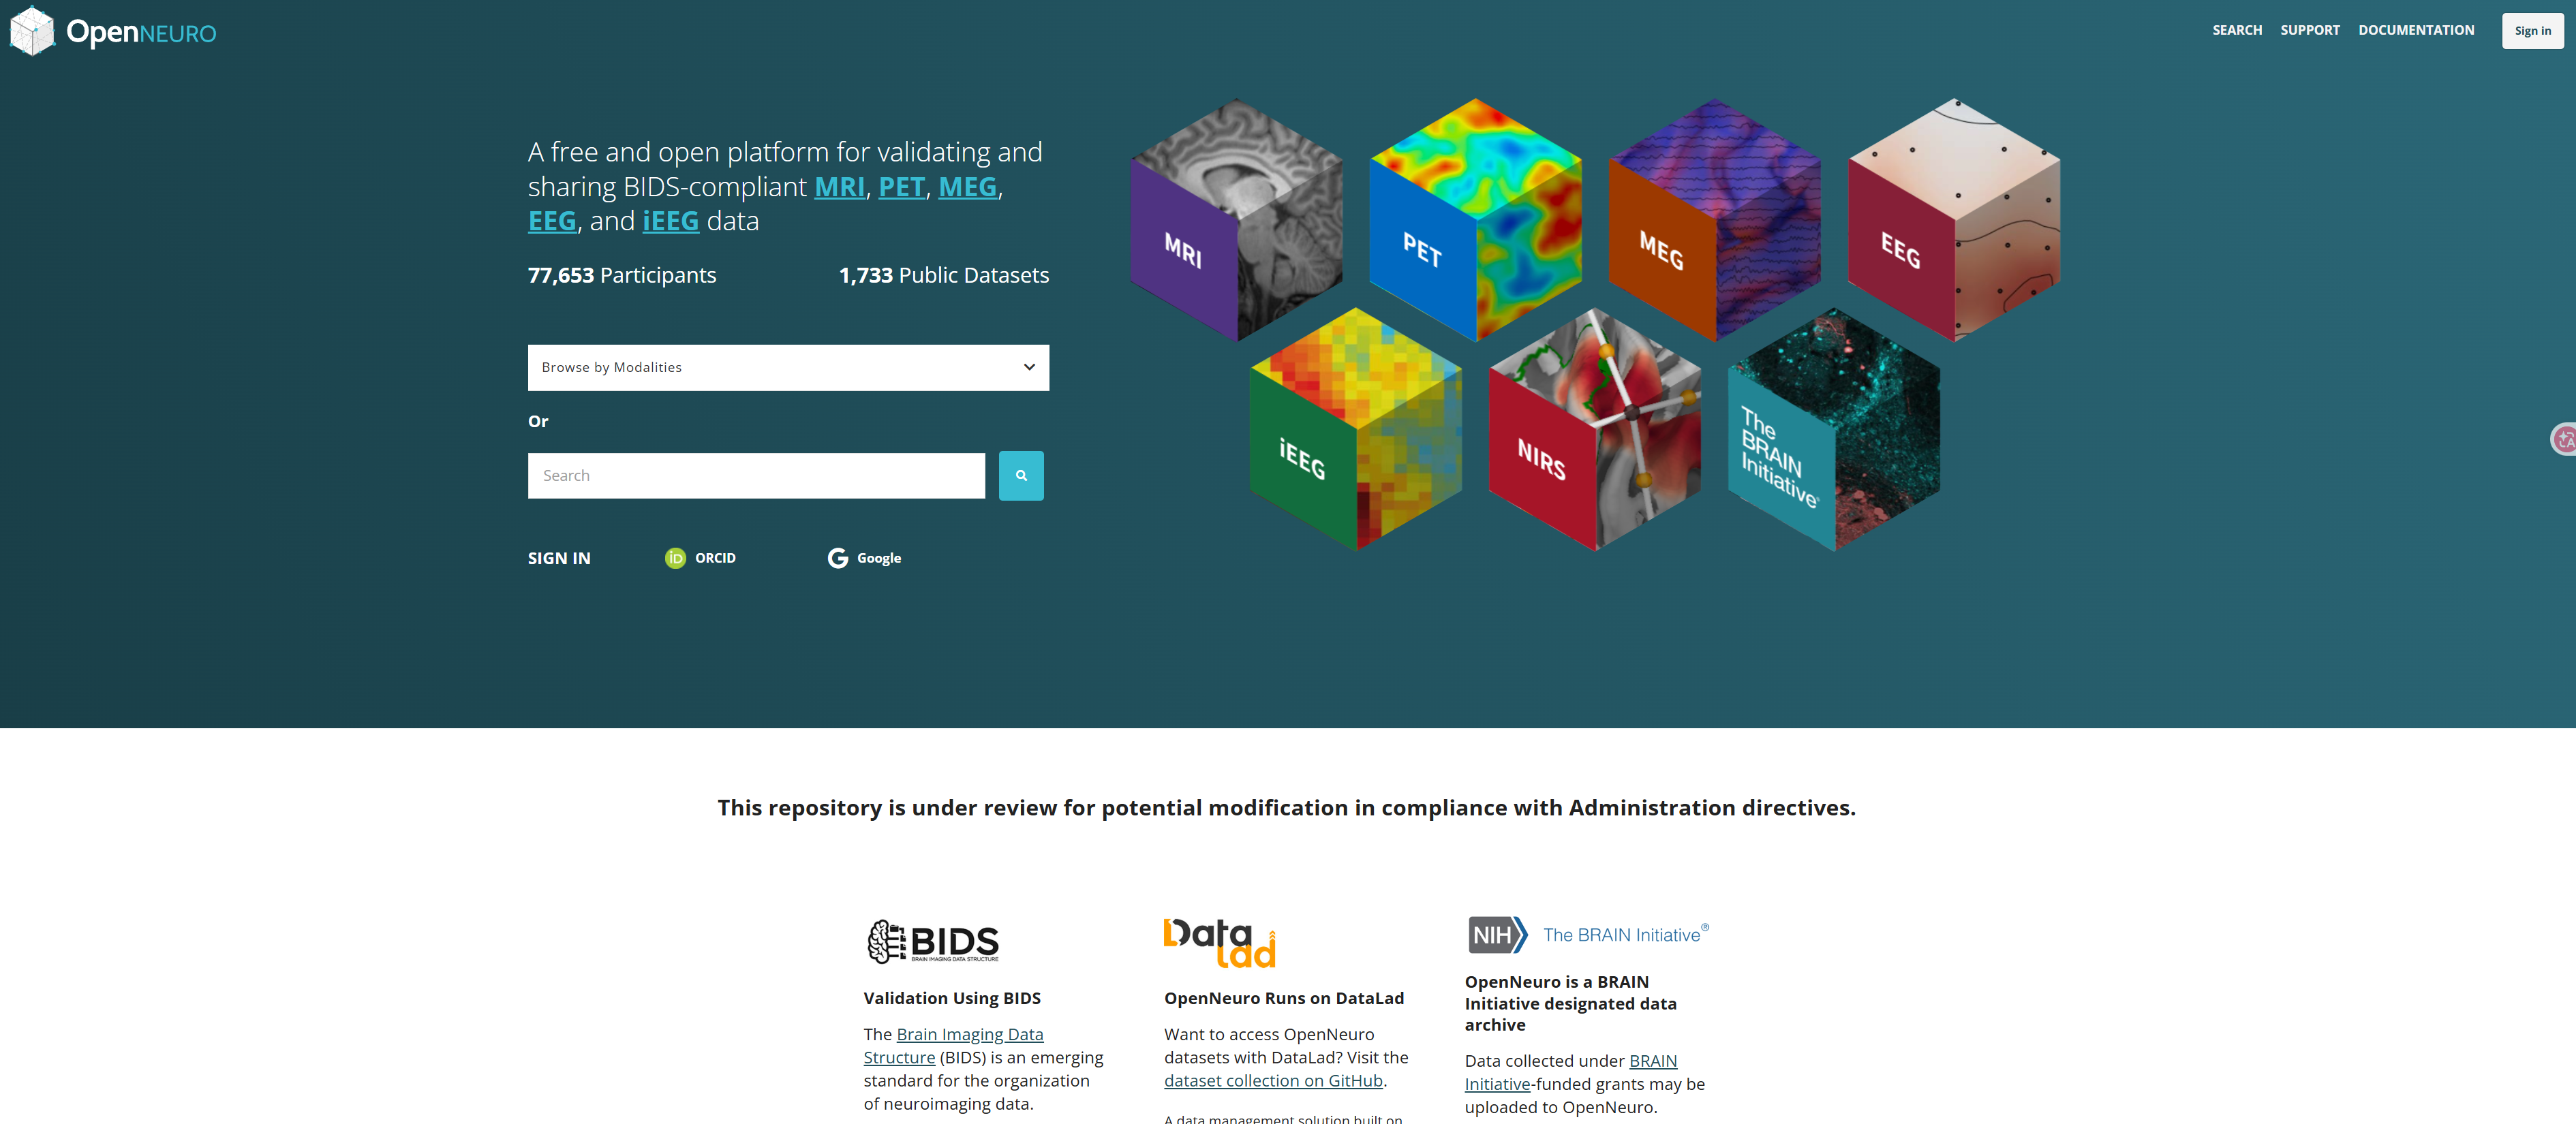
\includegraphics[width=0.85\textwidth]{figures/02_openneuro.png}
  \caption{OpenNeuro 平台界面}
  \label{fig:openneuro-ui}
\end{figure}

\subsubsection{国内分析}

在国内，EEG 数据管理的工具生态尚不成熟。多数实验室仍依赖通用的文件管理工具（如 Windows 资源管理器、坚果云同步盘）或科研协作平台（如问卷星用于知情同意收集、微信用于审批沟通）的``拼凑式''方案，缺乏专门针对 EEG 数据特点的整合性解决方案。

在医疗级系统方面，国内部分三甲医院和医疗器械厂商开发了脑电工作站软件（如 Nicolet、Natus 等品牌的配套系统），具备临床级别的数据采集与分析能力。但这类系统价格昂贵（通常以数十万元计），部署环境要求高（需专用服务器和网络），且聚焦于临床诊断而非科研管理，功能设计与教学科研场景的契合度较低。

在科研数据管理平台方面，国内部分高校开始建设科研数据中台或数据仓库，但这些平台多面向大规模、多学科的通用数据管理需求，对 EEG 等特定模态数据的元数据标准、质控规则和伦理审核流程缺乏领域针对性的支持。

\subsubsection{对比与借鉴}

综合以上分析，本系统的设计借鉴了以下先进理念：

\begin{itemize}
  \item 从 \textbf{EEGLAB} 和 \textbf{MNE-Python} 借鉴了 EEG 数据解析与质控的核心算法思路，但在实现上摒弃 MATLAB/Python 命令行的交互方式，提供 Web 图形化操作界面。
  \item 从 \textbf{OpenNeuro} 借鉴了 BIDS 标准化的数据组织理念，将其核心元数据规范融入系统的数据模型设计中。
  \item 从 \textbf{MNE-Python} 借鉴了开源和可复现性的理念，确保系统的数据处理流程透明、可追溯。
\end{itemize}

本系统与上述方案的核心差异在于：上述工具定位于``专业级分析''或``数据共享仓库''，而本系统填补的是``教学与基础科研场景下的数据管理与伦理管理系统''这一细分领域的空白。本系统不追求算法的极致丰富性，而是聚焦于数据治理的完整闭环——从数据入库到归档的全流程管理，以及从知情同意到操作审计的全链路伦理合规。

\subsection{用户需求}

本节根据系统三类核心用户角色分别阐述其需求，需求描述结合真实科研教学场景进行具体化说明。

\subsubsection{被试者}

被试者是 EEG 数据的来源主体，其核心诉求在于对个人数据使用的知情权和控制权。

\begin{itemize}
  \item 注册账号并等待管理员审批激活，登录后查看和修改个人基本信息。
  \item 在线阅读知情同意书模板，理解数据采集目的、使用范围和隐私保护措施后，完成电子化签署；对于已签署的知情同意书，有权在合理条件下撤回。
  \item 查看与本人相关的数据使用授权记录，了解哪些实验员在什么时间范围内、基于什么目的获得了本人数据的访问权限。
  \item 对已发放的数据使用授权进行撤回操作，撤回后系统应立即停止相关数据的后续访问，并通知相关实验员。
  \item 接收系统推送的站内通知，及时了解数据审核进展、授权状态变更和系统公告。
\end{itemize}

\subsubsection{实验员}

实验员是 EEG 数据的主要生产者和使用者，其核心诉求在于高效的数据管理、可靠的质控保障和便捷的分析工具。

\begin{itemize}
  \item 注册账号并等待管理员审批激活，登录后维护个人资料。
  \item 创建实验项目，录入实验名称、描述、用途类型（教学 / 科研）和时间范围等元数据，并在实验生命周期内维护其状态。
  \item 上传 EEG 原始数据文件（支持 CSV、EDF 等常见格式），填写或补充数据描述、采集设备信息和通道配置等元数据，并为数据添加自定义标签以便分类检索。
  \item 在数据上传后自动获得系统的解析与质控结果，包括文件格式校验、采样率一致性检测、通道完整性评估、缺失值比例和异常值统计，以及综合质控评分。
  \item 对质控通过的数据提交使用申请，说明使用目的、所需访问范围（查看 / 下载 / 分析）和期望的导出格式。
  \item 在获得有效授权后，对 EEG 数据执行时域波形可视化、统计摘要、FFT 频谱分析、频段能量计算和 AI 状态识别等分析任务，并下载分析结果。
  \item 对已归档或不再使用的数据执行冻结或归档操作，参与数据的全生命周期管理。
\end{itemize}

\subsubsection{管理员}

管理员是系统的运维与合规保障者，其核心诉求在于维护系统秩序、把控合规底线和保障运行安全。

\begin{itemize}
  \item 审批新注册用户（被试者和实验员）的账号申请，对不符合条件的注册予以驳回，对已激活的账号进行禁用或恢复操作。
  \item 审核实验员上传的 EEG 数据，基于系统自动生成的质控报告做出审核通过或驳回的决定，并给出审核意见。
  \item 审批实验员提交的数据使用申请，基于知情同意签署情况和数据敏感程度决定是否授权，基于伦理审查规范进行授权投票，指定授权的访问范围和有效期限。
  \item 创建和维护知情同意书模板，管理模板的版本控制——系统同时仅允许一个 Active 版本生效，历史版本保留备查。
  \item 查看系统操作审计日志，按操作人、操作类型、对象类型和时间范围进行筛选和追溯，监控异常操作行为。
  \item 维护系统运行配置参数，包括上传文件大小上限、支持的文件格式列表、Token 有效期、验证码有效期和日志保留时长等。
  \item 接收系统异常告警通知，及时响应数据处理失败、存储空间不足等运维事件。
\end{itemize}
